% This program can be redistributed and/or modified under the terms
% of the GNU Public License, version 3.
%
% Seth Brown, Ph.D.
% sethbrown@drbunsen.org
%
% Compiled with XeLaTeX
% Dependencies:
%   Fontin Sans font (http://www.exljbris.com/fontinsans.html)
%
%\documentclass{beamer}
\documentclass[unknownkeysallowed]{beamer}

\usepackage{graphicx} % graphics
\usepackage{epsfig} % eps graphics
\usepackage{hyperref} % urls
\usepackage{booktabs, caption} % table styling

% suppress navigation bar
\beamertemplatenavigationsymbolsempty


\mode<presentation>
{
  \usetheme{bunsen}
  \setbeamercovered{transparent}
  \setbeamertemplate{items}[circle]
}

% set fonts
\usepackage{fontspec}
\setsansfont{Ubuntu}
\setbeamerfont{frametitle}{size=\LARGE,series=\bfseries}

% color definitions
\usepackage{color}
\definecolor{uipoppy}{RGB}{225, 64, 5}
\definecolor{uipaleblue}{RGB}{96,123,139}
\definecolor{uiblack}{RGB}{0, 0, 0}

% caption styling
\DeclareCaptionFont{uiblack}{\color{uiblack}}
\DeclareCaptionFont{uipoppy}{\color{uipoppy}}
\captionsetup{labelfont={uipoppy},textfont=uiblack}
\setbeamercolor{section in toc}{fg=uipoppy}

% see the macros.tex file for definitions
% This program can be redistributed and/or modified under the terms
% of the GNU Public License, version 3.

% adds reference to bottom right of corner of a slide
\usepackage[absolute,overlay]{textpos} % text references in slide corners
\newcommand\textref[1]{%
  \begin{textblock*}{\paperwidth}(0pt,0.99\textheight)
  \raggedleft \tiny{\emph{#1}}\hspace{.5em}
  \end{textblock*}}

  %font size
  \newcommand\Fontvi{\fontsize{6}{7.2}\selectfont}
  \newcommand\Fontix{\fontsize{9}{11}\selectfont}

% for drawing circles around numbers
% ex. \circled{1} Add some text here.
\usepackage{tikz}
\newcommand*\circled[1]{\tikz[baseline=(char.base)]{
            \node[shape=circle,draw,inner sep=2pt] (char) {#1};}}



% title slide definition
\title{Security of Near Field Communication:\break Does My Phone Need A Tinfoil Hat?}
\author{Thomas Harren}
\institute[UMM] % (optional, but mostly needed)
{
 % \inst{1}%
  University of Minnesota, Morris
}
\date[]{April 30, 2015}

%--------------------------------------------------------------------
%                    Introduction & Outline
%--------------------------------------------------------------------

\begin{document}

\begin{frame}
  \titlepage
\end{frame}

% Set the background for the rest of the slides.
% Insert infoline
\setbeamertemplate{background}
 {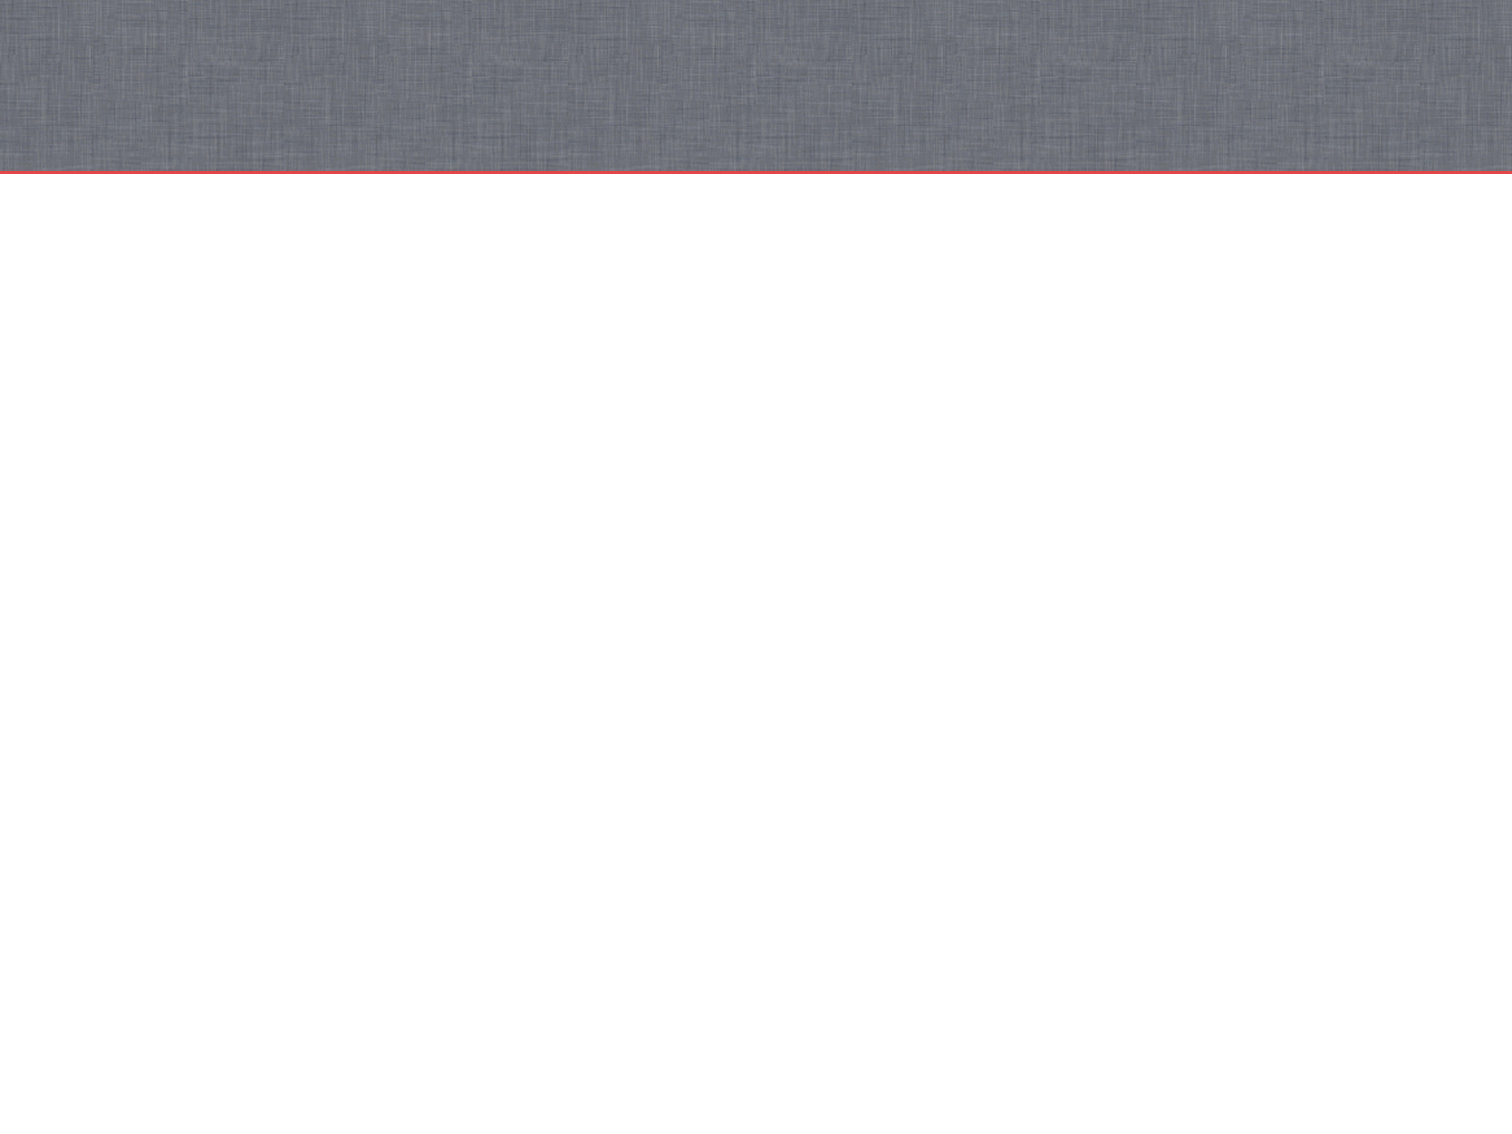
\includegraphics[width=\paperwidth,height=\paperheight]{slide_bg}}
\setbeamertemplate{footline}[bunsentheme]


\begin{frame}
\frametitle{Have you used NFC?}
  \begin{columns}[T]
    \begin{column}{.5\textwidth}
  		\begin{block}{}
  		  \begin{center}
    		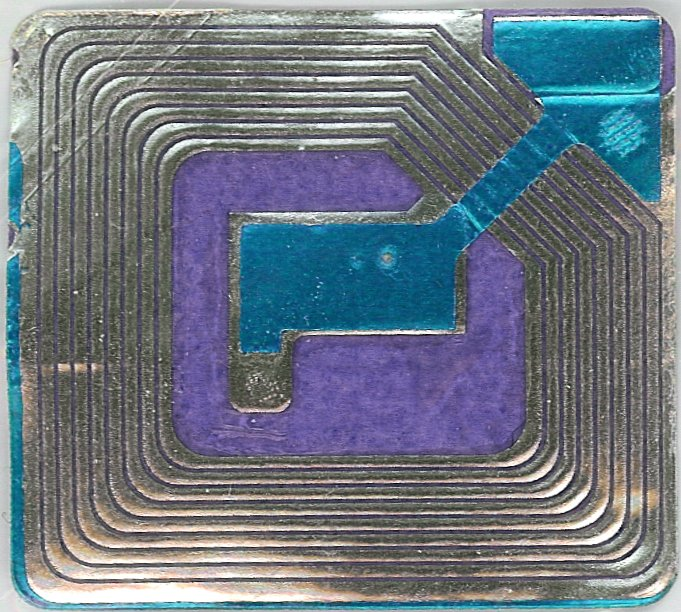
\includegraphics[scale=.5]{figures/wikimediatag.jpg}
    		\end{center}
    	\end{block}
    \end{column}
    \begin{column}{.5\textwidth}
        test
    \end{column}
  \end{columns}
  \textref{Image from wikipedia commons}
\end{frame}

\begin{frame}
  \frametitle{Outline}
    \begin{center}\begin{minipage}{.9\textwidth}
        \tableofcontents[
          currentsection,
          sectionstyle=show/show,
          subsectionstyle=show/shaded/hide
        ]
    \end{minipage}\end{center}
 \end{frame}


\Fontix

%-------------------------------------------------------------------
%                           Section
\section{Background}
\begin{frame}
  \frametitle{Background}
    \begin{center}\begin{minipage}{.9\textwidth}
    \tableofcontents[currentsubsection, hideothersubsections, sectionstyle=show/shaded]
    \end{minipage}\end{center}
\end{frame}
%
%-------------------------------------------------------------------


\subsection{Elements of HF RFID: Tags \& Readers}
\begin{frame}
\frametitle{Tags \& Readers}

  \begin{columns}[T]
    \begin{column}{.5\textwidth}
  		\begin{block}{}
  		  	\begin{center}
  			NFC is built using from elements of \textit{high-frequency radio frequency identification} (HF RFID).
  			\newline
  			\newline
    		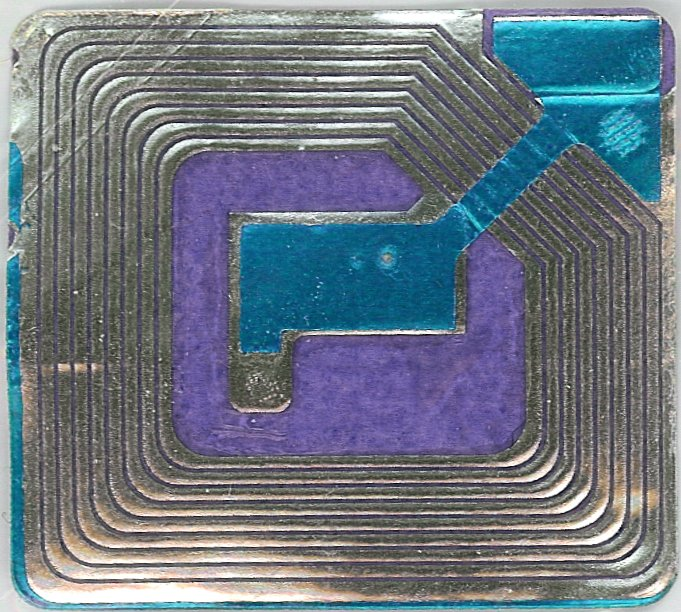
\includegraphics[scale=.5]{figures/wikimediatag.jpg}
    		\end{center}
    	\end{block}
    \end{column}
    \begin{column}{.5\textwidth}
        \begin{block}{Tag}
		\begin{itemize}
		    \item{A tiny circuit with an antenna coil}
		    \item{Stores limited information}
		    \item{Can be powered or passive}
        	\item{Passive tags are smallest and cheapest}
   		\end{itemize}
    	\end{block}
        \begin{block}{Reader}
    	\begin{itemize}
		    \item{Reader emits electricity using an antenna coil}
		    \item{Initiates communication}
   		\end{itemize}
    \end{block}
    \end{column}
  \end{columns}
  \textref{Image from wikipedia commons}
\end{frame}

\begin{frame}
  \frametitle{Physics: Electromagnetic Induction}
\end{frame}
%%%reset slide%%%
\begin{frame}
\frametitle{\textcolor{uipoppy}{Physics:} Electromagnetic Induction}
  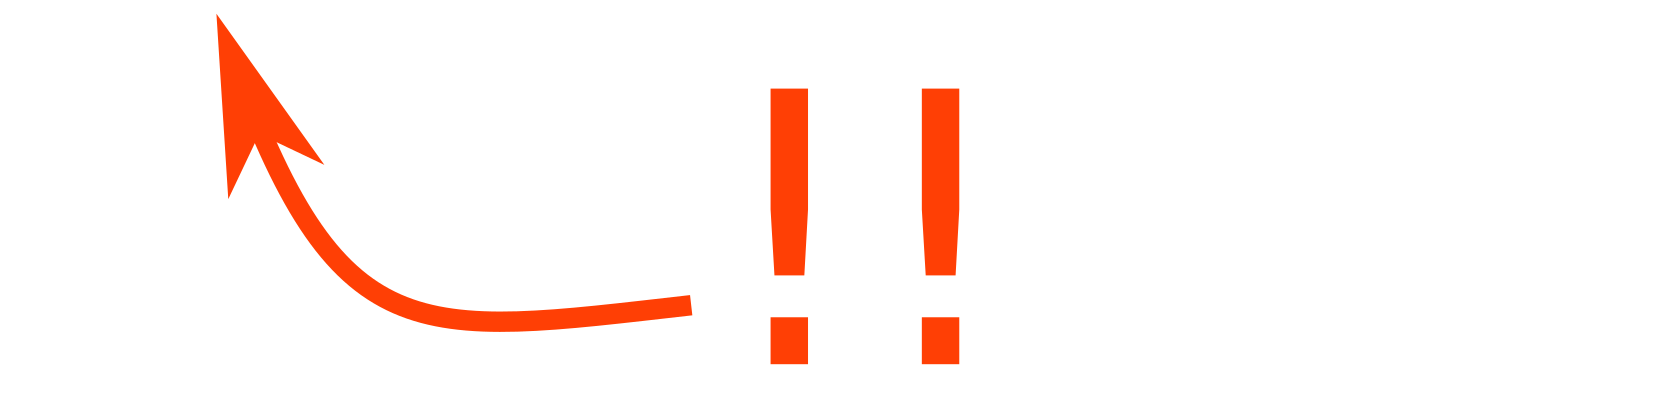
\includegraphics[scale=.5]{figures/arrow.png}
  \begin{center}\begin{minipage}{.9\textwidth}
     \begin{block}{Tom, this is a computer science presentation, \newline not physics. Why...?}
     	%But its pretty neat stuff.
     \end{block}
  \end{minipage}\end{center}
\end{frame}
%%%reset slide%%%
\begin{frame}
\frametitle{Physics: Electromagnetic Induction}
  \begin{center}\begin{minipage}{.9\textwidth}
    %To show very quickly
     \begin{block}{But its physics, and scary...}
     \end{block}
  \end{minipage}\end{center}
\end{frame}
%%%reset slide%%%
\begin{frame}
\frametitle{Physics: Electromagnetic Induction}
  \begin{center}\begin{minipage}{.9\textwidth}
  NFC and RFID uses \textit{electromagnetic induction}, the same technology used in power transformers \newline
  \begin{columns}[T]
  \begin{column}{.5\textwidth}
    \begin{block}{}\begin{center}
      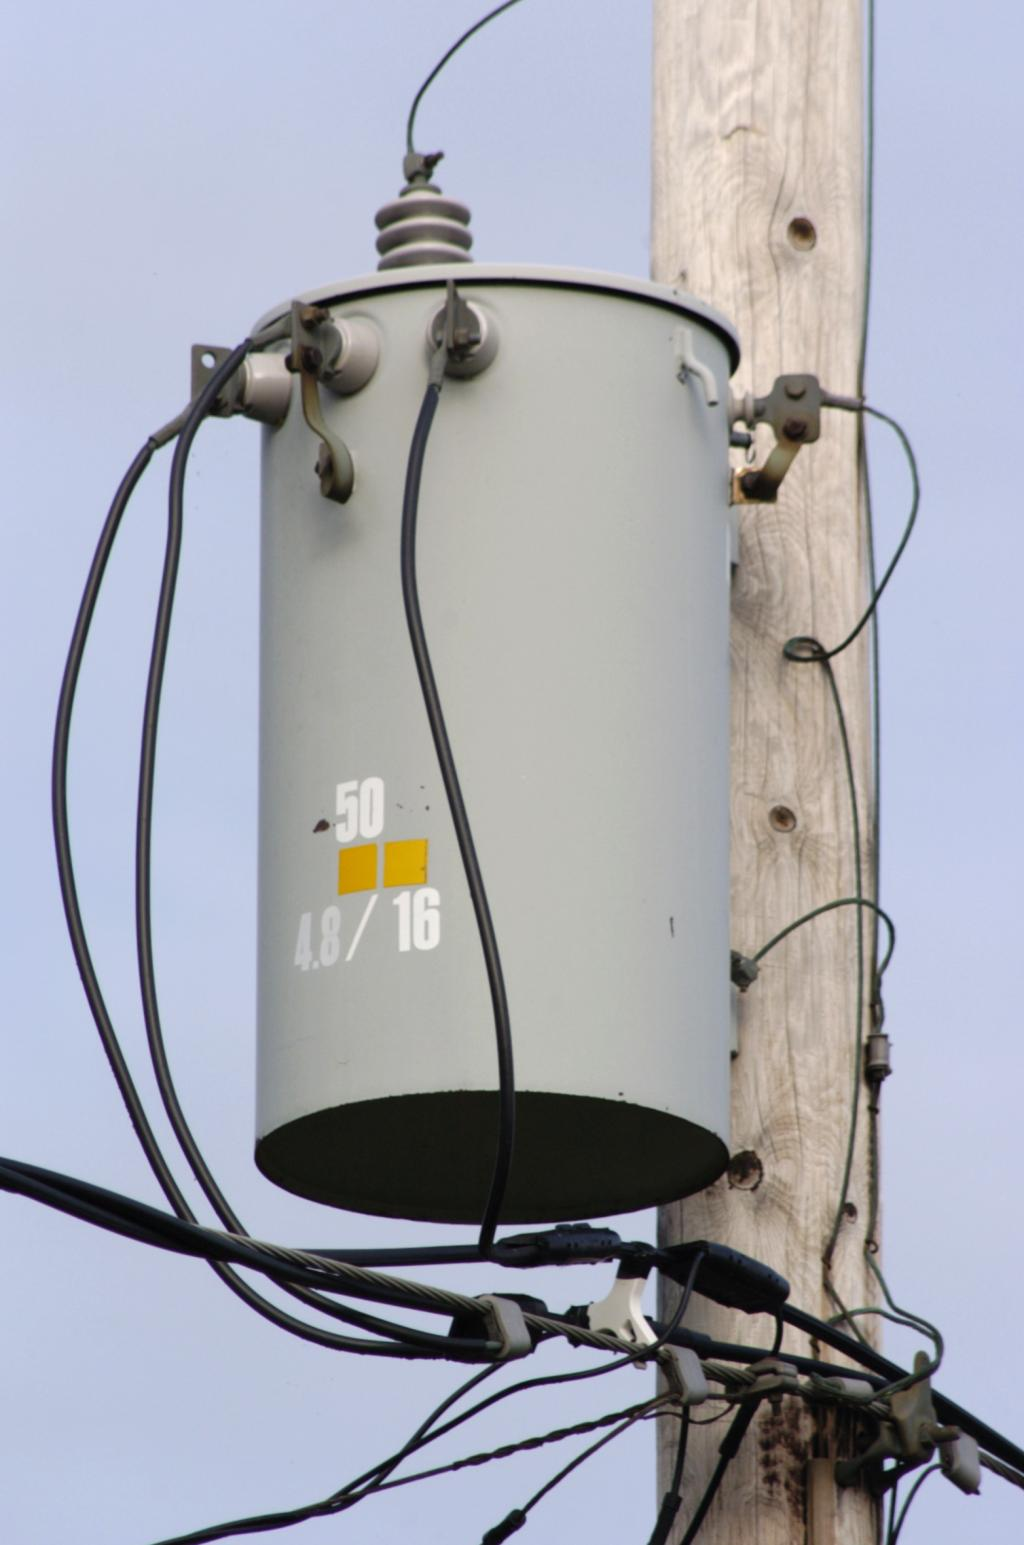
\includegraphics[width=0.2\paperwidth]{figures/Polemount-singlephase-closeup.jpg}
    \end{center}\end{block}
  \end{column}
    \begin{column}{.5\textwidth}
      \begin{block}{}\begin{center}
        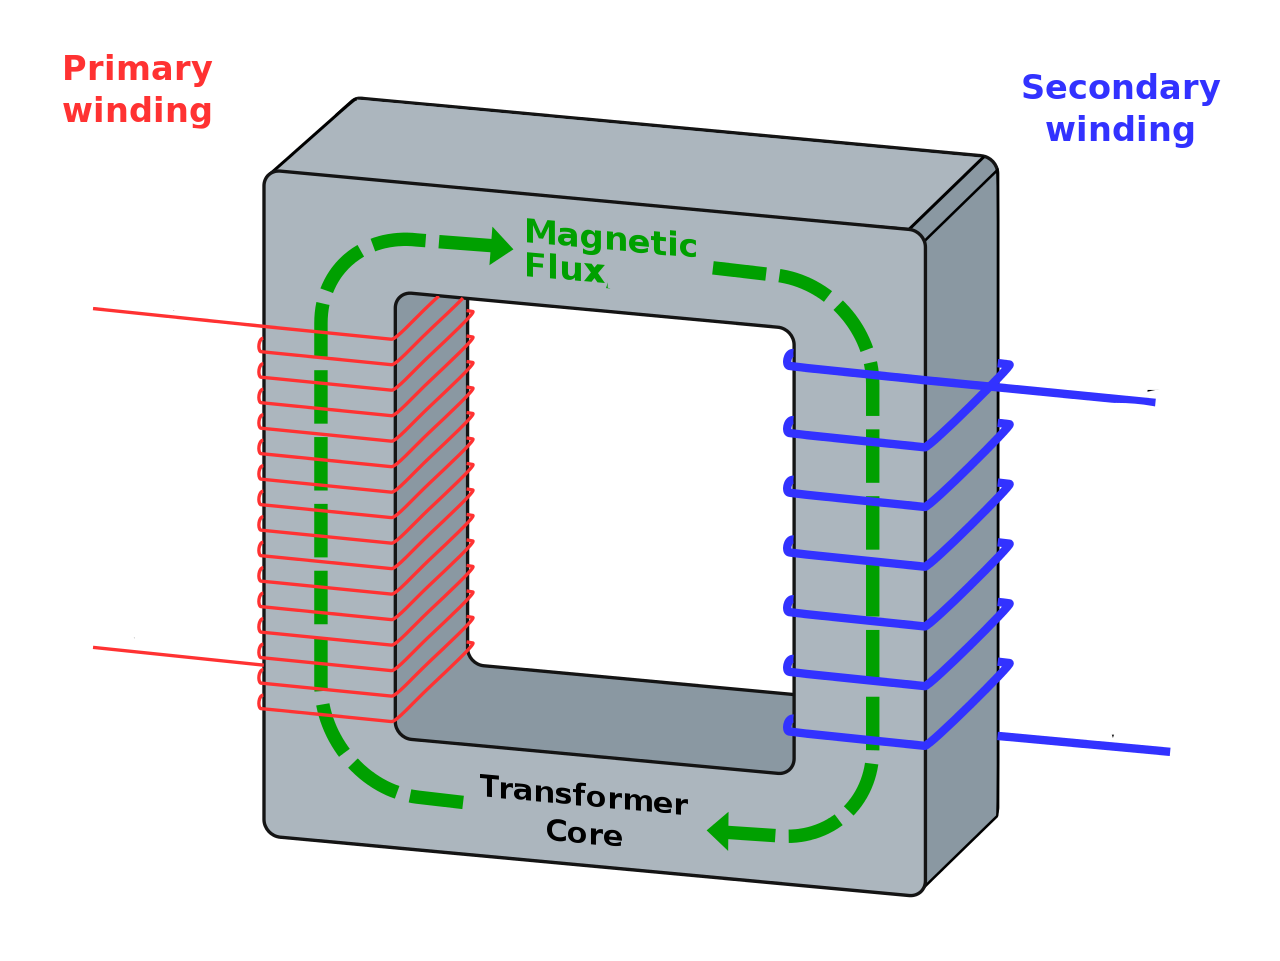
\includegraphics[width=0.4\paperwidth]{figures/solidcore.png}
      \end{center}\end{block}
    \end{column}
  \end{columns}
  \end{minipage}\end{center}
  \textref{Images originate from "Transformers" wikipedia page}
\end{frame}


\begin{frame}
\frametitle{Basic NFC Communication}
  \begin{center}\begin{minipage}{.9\textwidth}
  \begin{columns}[T]
    \begin{column}{.5\textwidth}
     \begin{block}{HF RFID Communication}
		\begin{enumerate}
		    \item{Reader emits electricity}
		    \item{Tag is activated by induced power}
        	\item{Reader runs discovery protocol, selecting tag by unique ID}
        	\item{Communication ensues}
   		\end{enumerate}
    \end{block}
         \begin{block}{Features}
		\begin{itemize}
        	\item{Quick setup}
        	\item{Line of sight not required}
   		\end{itemize}
    \end{block}
    \end{column}
    \begin{column}{.5\textwidth}
    \begin{block}{}
     \begin{center}
     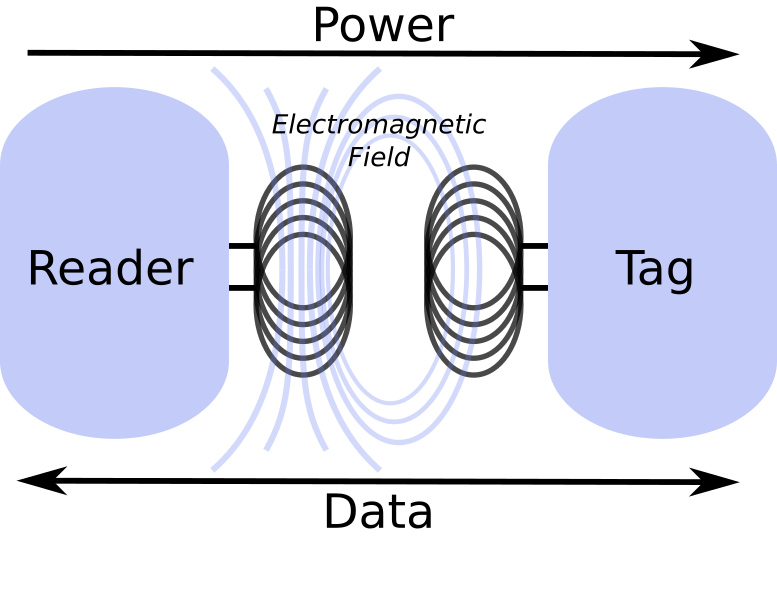
\includegraphics[width=0.4\paperwidth]{figures/emitterAndTag.png}
     \end{center}
    \end{block}
    \end{column}
  \end{columns}
  \end{minipage}\end{center}
\end{frame}


\subsection{NFC on Mobile Phones}

\begin{frame}
\frametitle{NFC is Fancy HF RFID}
  \begin{center}
  \begin{minipage}{.7\textwidth}
  \begin{block}{NFC adds a few features to HF RFID:}
		\begin{enumerate}
		  \item{Phone can act as readers}
		  \item{Phones can emulate tags}
      \item{Phones can communicate peer-to-peer}
   	\end{enumerate}
  \end{block}
  \end{minipage}
  \end{center}
\end{frame}


\subsection{NFC and the Payment Industry}
\subsection{Security for NFC}

%-------------------------------------------------------------------
%                           Section
\section{Contactless Credit Cards}
\begin{frame}
  \frametitle{Contactless Credit Cards}
    \begin{center}\begin{minipage}{.9\textwidth}
    \tableofcontents[currentsubsection, hideothersubsections, sectionstyle=show/shaded]
    \end{minipage}\end{center}
\end{frame}
%
%-------------------------------------------------------------------
\subsection{Current Credit Card Protocol}
\subsection{Credit Card Attacks}
\subsection{Proposed Secure Credit Card Protocol}

%-------------------------------------------------------------------
%                           Section
\section{NFC and Mass Transit Ticketing}
\begin{frame}
\frametitle{NFC and Mass Transit Ticketing}
\begin{center}\begin{minipage}{.9\textwidth}
\tableofcontents[currentsubsection, hideothersubsections, sectionstyle=show/shaded]
\end{minipage}\end{center}
\end{frame}
%
%-------------------------------------------------------------------

\subsection{Ticketing Architecture}


%-------------------------------------------------------------------
%                           Section
\section{EnGarde: Physical NFC Security}
\begin{frame}
\frametitle{EnGarde: Physical NFC Security}
\begin{center}\begin{minipage}{.9\textwidth}
\tableofcontents[currentsubsection, hideothersubsections, sectionstyle=show/shaded]
\end{minipage}\end{center}
\end{frame}
%
%-------------------------------------------------------------------

\subsection{No Power Mode}
\subsection{System Idle Mode}
\subsection{NFC Decoder Active Mode}
\subsection{Jam Mode}
\subsection{Experimental Evaluation of EnGarde}


%-------------------------------------------------------------------
%                           Section
\section{Conclusion}
\begin{frame}
\frametitle{Conclusion}
\begin{center}\begin{minipage}{.9\textwidth}
\tableofcontents[currentsubsection, hideothersubsections, sectionstyle=show/shaded]
\end{minipage}\end{center}
\end{frame}
%
%-------------------------------------------------------------------
\begin{frame}
  \frametitle{Conclusion}
  \begin{block}{Tinfoil Hats for Everyone!}
  \end{block}
\end{frame}

\begin{frame}
  \frametitle{Sources}
  \begin{block}{Primary Research Sources}
    \begin{enumerate}
      \item{Oliver Jensen, Mohamed Gouda, and Lili Qiu. 2016. A secure credit card protocol over NFC. In Proceedings of the 17th International Conference on Distributed Computing and Networking (ICDCN '16). ACM, New York, NY, USA, Article 32 , 9 pages. %DOI=http://dx.doi.org.ezproxy.morris.umn.edu/10.1145/2833312.2833319
      }
      \item{Sandeep Tamrakar, Jan-Erik Ekberg, and N. Asokan. 2011. Identity verification schemes for public transport ticketing with NFC phones. In Proceedings of the sixth ACM workshop on Scalable trusted computing (STC '11). ACM, New York, NY, USA, 37-48. %DOI=http://dx.doi.org.ezproxy.morris.umn.edu/10.1145/2046582.2046591
      }
      \item{Jeremy J. Gummeson, Bodhi Priyantha, Deepak Ganesan, Derek Thrasher, and Pengyu Zhang. 2013. EnGarde: protecting the mobile phone from malicious NFC interactions. In Proceeding of the 11th annual international conference on Mobile systems, applications, and services (MobiSys '13). ACM, New York, NY, USA, 445-458. %DOI=http://dx.doi.org.ezproxy.morris.umn.edu/10.1145/2462456.2464455
      }
    \end{enumerate}
  \end{block}
\end{frame}


%-------------------------------------------------------------------
%                          Sample Slide
%-------------------------------------------------------------------

%\begin{frame}
%    \frametitle{Elements in Whoville}
%
%    \vspace{1cm} % generate some space between title and content
%    \begin{table}[h]
%    \centering
%    \begin{tabular}{lcccc} \bottomrule[2pt]
%        Name & Symbol & $A_r$ & M.P. (K) & IE (J) \\ \bottomrule
%        Helium & He & $4.00$ & $1$ & $3.94e^{-18}$ \\
%        Carbon & C & $12.01$ & $773$ & $3.94e^{-18}$ \\
%        Arsenic & As & $74.92$ & $1090$ & $1.48e^{-18}$ \\
%        Gold & Au & $196.96$ & $1337$ & $1.48e^{-18}$ \\
%        Cobalt & Co & $58.93$ & $1495$ & $1.26e^{-18}$ \\
%    \bottomrule[2pt]
%    \end{tabular}
%    \caption{Properties of Whoville Elements}
%    \end{table}
%
%\vspace{-0.6cm} % compact spacing between table and text
%
%    \begin{columns}[t]
%    \column{4.5cm}
%    \begin{block}{Trace rare earth metals:}
%    \begin{itemize}
%        \item{Ytterbium}
%        \item{Praseodymium}
%        \item{Neodymium}
%    \end{itemize}
%    \end{block}
%    \column{4.5cm}
%    \begin{block}{Obtaining Neodymium:}
%        \vspace{0.15cm}
%        \circled{1}$\textemdash$bastn\"{a}site \\
%        \circled{2}$\textemdash${monazite} \\
%    \end{block}
%    \end{columns}
%
%    \textref{Dr. Seuss et al. 2011}
%
%\end{frame}

\end{document}
